\chapter{Introduction}
\label{Introduction}

Audio processing has been of interest since the [wtd since when has audio processing been of interest?].  Mainly, audio processing was used in [wtd what was audio processing used in].  Before computers, audio processing was handled via discrete circuits [wtd or whatever the history of audio processing was].  Audio processing consists of several different areas [wtd list areas that audio processing consists of, for example audio classification is one of them].

One of the more interesting areas of audio processing is audio classification.  Given an audio sample, choose the best-fit class for that sample from a finite set of classes.  For example, in music genre classification, the task is to choose which genre a music sample belongs to.  In our paper, we specifically look at urban sound classification: given an audio sample, choose which class, for example, shouting, car horns, or other sounds that occur in natural urban environments, the sample belongs to.  This problem has several applications such as [wtd include audio classification applications].

Machine learning can be of great use in the field of audio processing.  Previously, however, machine learning has only seen popularity in the audio processing task of speech recognition.  While there have been many advances in this area, there has been less work in other audio processing tasks, for example, in the detection of urban sounds and audio classification in general.  Until recently, these tasks have been approached using sophisticated, hand-crafted features and algorithms that have existed since the sixties or earlier.  These algorithms were optimized to take advantage of analog hardware.  As hardware advanced, more modern algorithms and techniques were able to be used such as gradient boosting and neural networks.  These approaches represent the current state-of-the-art as it applies to audio classification.

The purpose of this thesis is to apply state-of-the-art neural network architectures and feature extraction to the task of urban sound classification using the dataset SONYC [wtd cite and use the correct name].  In this regard, we discuss several popular neural network architectures, such as CNNs, LSTMs, and attention mechanisms, and their performance in regards to audio classification.  We specifically explore the use of LSTMs in urban sound classification, both with and without attention mechanisms.  Furthermore, we explore and compare this to the use of gradient boosting against the same dataset.

\chapter{Background and Related Work}
\label{Background and Related Work}

\section{Machine Learning and Audio Processing Tasks}

[wtd list and describe various audio processing task such as sound classification and speech recognition]

[wtd describe historical approaches to audio classification and audio processing tasks]

\section{Linear and Logistic Regression}

[wtd explain what it is, advantages such as linearly separable data, disadvatnages]

The primary downfall of linear/logistic regression is the inability to model non-linear relationships. [wtd explain this further]

\section{SVMs}

Support vector machines (SVM) are... [wtd explain how support vector machines work].  SVMs have shown great success in the classification of high-dimensional data.

[wtd explain how kernel trick works]

[wtd, explain the what the pitfalls of SVMs are, such as choosing a kernel, citations needed]

\section{Random Forests}

[wtd explain how random forests work, include some math figures]

[wtd explain advantages of random forests, such as speed of training, higher accuracy on smaller dimensional data or datasets]

[wtd explain pitfalls of random forests]

\subsection{Gradient Boosting}

Gradient boosting is an supervised ensemble learning method that combines many "weak" learners, to form one single strong learner.  It has been proven to be a very successful machine learning method, has been applied with great success to many different Kaggle challenges (a machine learning competition).  It can be applied to both regression and classification problems.

[wtd explain gradient boosting, make sure to cite XGBoost and Adaboost papers]

[wtd explain advantages of gradient boosting]

[wtd explain disadvantages of gradient boosting]

\section{Neural Networks}

Contrary to the previously discussed approaches to machine learning, neural networks have existed for much longer [wtd cite Pitts and McCulloch the first neural network paper].  Neural networks have had a fickle history as well, with an ebb-and-flow of popularity, last peaking in the 90s [wtd cite some papers about NNs from Bengio, etc.].  Due to advances in computational power, parallel processing paradigms, and neural network architectures in the past several years, neural networks are seeing great successes across many machine learning tasks.  For example, in [wtd example task like MNIST or anything that had breakthrough results cite paper] neural networks were able to perform at a level previously thought not possible.  [wtd explain what neural networks are, put graphs, explain advantages such as ability to deal with curse of dimonsionality and ability to deal with non-linear relationships, explain pitfalls]. [wtd explain stochastic gradient descent and optimizers ADAM, Adadelta, momentum, etc.]

\subsection{Activation Functions}

After each neuron has calculated the sum of its weighted inputs, it passes it to a (usually non-linear) "activation" function.  There are advantages and disadvantages to different activation functions.


\subsubsection{Linear}

A linear activation function takes the weighted summed inputs to the neuron and multiplies it by a constant, giving the neuron the ability to scale the inputs.

{\centering
  $f(x)=cx$\par
}


\subsubsection{Sigmoid}
[wtd describe sigmoidal activation, include math]

{\centering
	$\displaystyle f(x)={\frac {L}{1+e^{-k(x-x_{0})}}}$\par
}

\subsubsection{TanH}

Similar to the sigmoid function, [wtd explain tanh]

\subsubsection{Rectified Linear Unit}
[wtd describe relu activation, include math]

{\centering
	$f(x)=max(0, x)$\par
}

\subsubsection{Scaled Exponential Linear Unit}
[wtd describe selu activation, include math, include special initialization required]


{\centering
	$\text{selu}(x) = \lambda\ \begin{cases}
    x,& \text{if } x > 0\\
    \alpha e^{x} - \alpha,& \text{if } x\leq 0\\
	\end{cases}$
	\par
}


The paper (\cite{DBLP:journals/corr/KlambauerUMH17})


\subsubsection{Softmax}
The softmax activation function transforms a set of probabilities

{\centering
	$\sigma (\mathbf {z} )_{j}={\frac {e^{z_{j}}}{\sum _{k=1}^{K}e^{z_{k}}}}$
	\par
}

\subsection{Convolutional Neural Networks}

Convolutional neural networks refers to any neural network with a convolutional layer.  These networks have achieved state-of-the-art results on many computer vision-related tasks, primarily because of their ability to "downsample" inputs while minimizing information loss.  It is because of this "downsampling" that these network are feasible to train, as opposed to a fully-connected network which has significantly more weights to train.  A convolutional layer is one that attempts to discover spatial relationships, aka filters, across neuronal inputs. [wtd describe + show graphs of convolutional layers].  This layer contains a set of filters, or weight matrices, that are convolved across the neuronal inputs, resulting in an output matrix called a feature map.  The weights of the filters are learned during training.  Typically these networks involve other spatial layers, such as max pooling layers, which directly downsample the neuronal inputs.

\subsection{Recurrent Neural Networks}

[wtd describe recurrent neural networks, cite original paper]

[wtd include math and graphs of basic RNN structure]

[wtd explain exactly the problem that RNNs solve (sequence and removing the need to include historical data in the inputs similar to how CNNs solve the problem of needing so many weights for the spatial input)]

While CNNS solve the problem of dimensionality in terms of spatial relationships, RNNs do so in terms of sequential, or temporal relationships.  Typically, to represent a temporal or sequential relationship, inputs are stacked in a windowed-fashion.  However, this greatly increases the number of weights required at the input layer.  Therefore, RNNs reduce the amount weights by allowing sequences to be passed in without requiring weights be connected to these input features.

\subsubsection{LSTMs}

\begin{figure}[h]
    \centering
	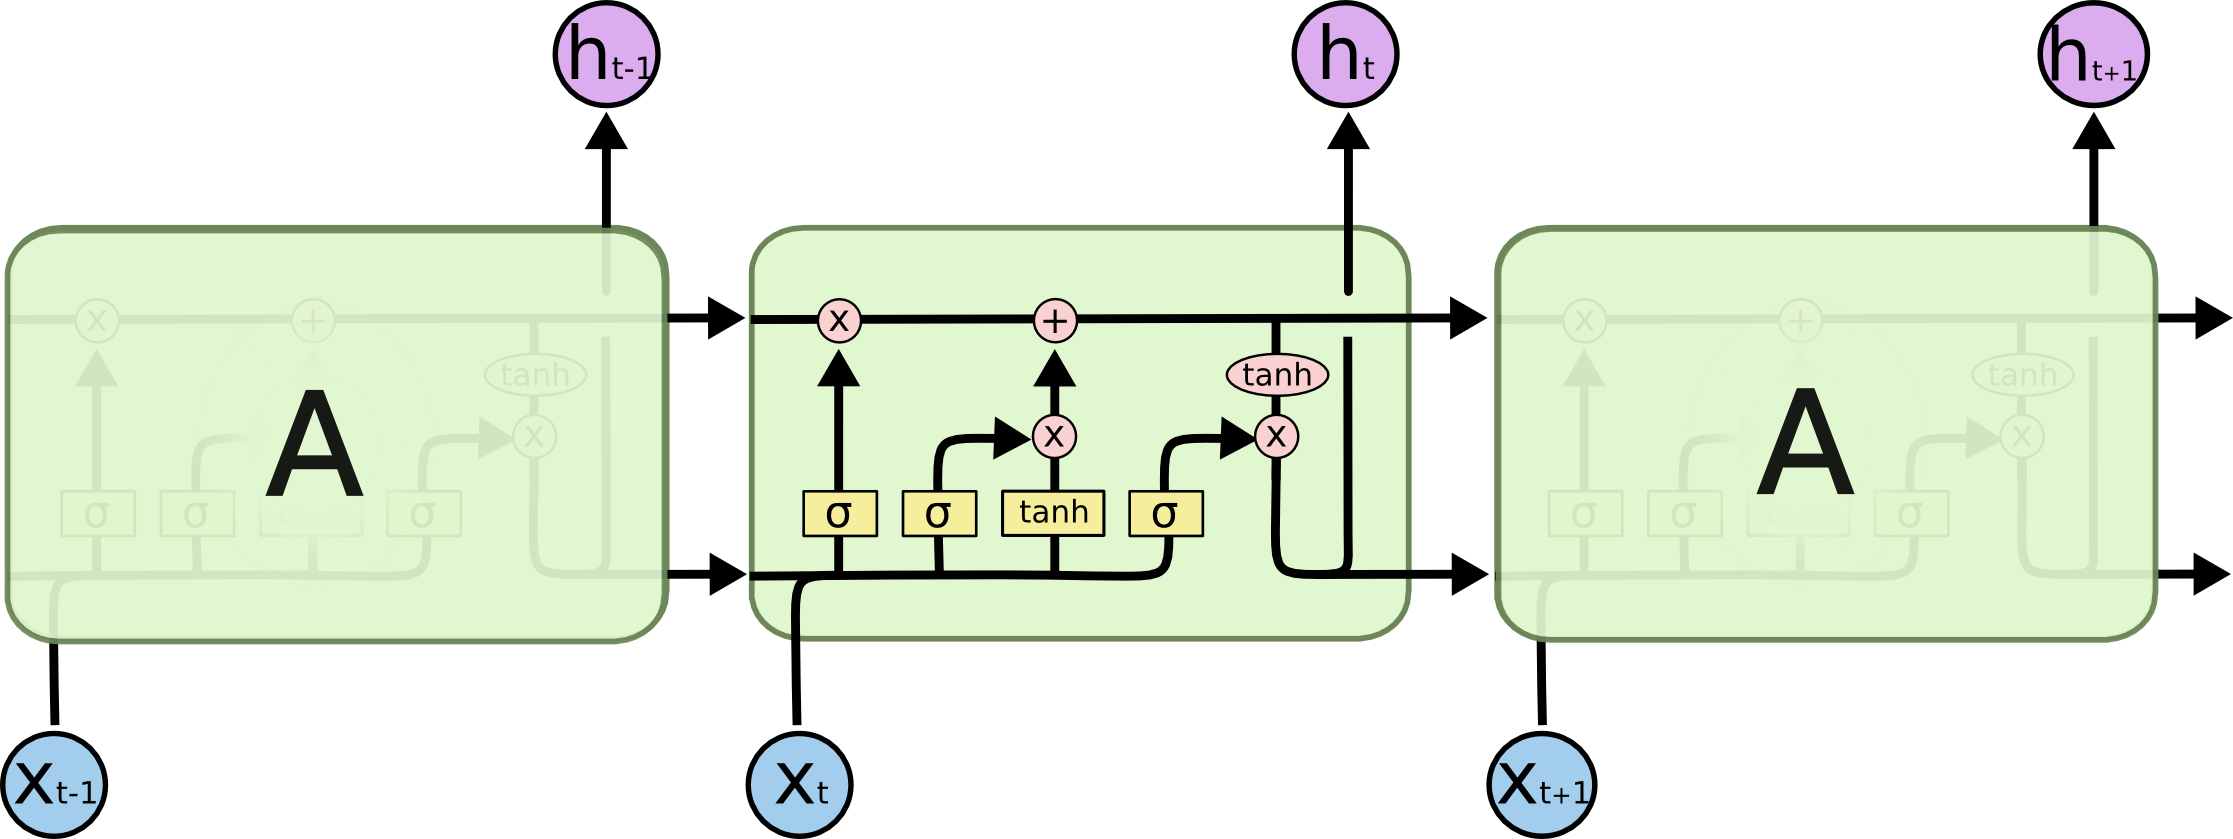
\includegraphics[width=.8\textwidth]{./images/illustrations/LSTM3}
    \caption{The repeating module in an LSTM contains four interacting layers.}
    \label{fig:mesh1}
\end{figure}\footnote{Source: http://colah.github.io/posts/2015-08-Understanding-LSTMs/. Reproduced with permission}





One of the pitfalls of recurrent neural networks is their inability to model [wtd describe lstms]

[wtd describe lstms and include graphs]

[wtd describe what problems lstms solve aka able to capture longer sequences, and downfalls]

\subsubsection{GRUs}

\begin{figure}[h]
    \centering
	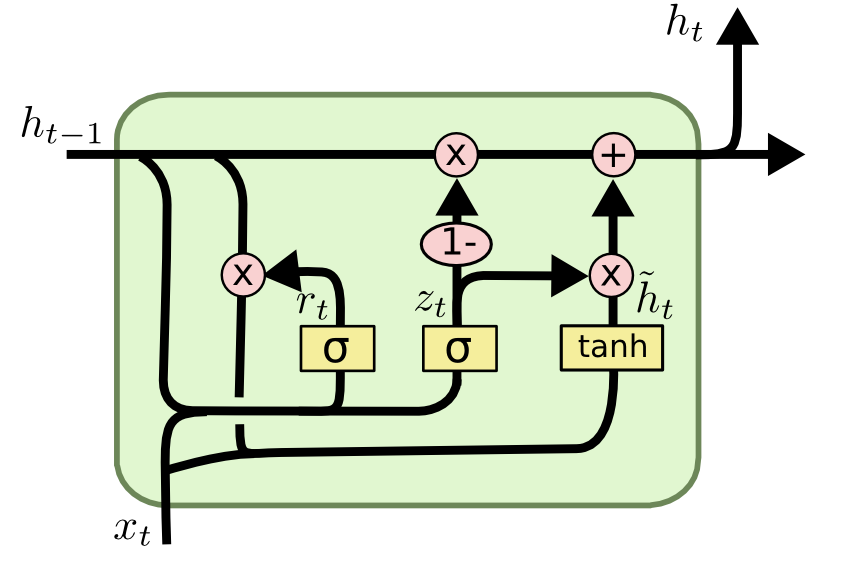
\includegraphics[width=.8\textwidth]{./images/illustrations/GRU}
    \caption{A GRU, as defined by Cho, et al. (2014).}
    \label{fig:mesh1}
\end{figure}\footnote{Source: http://colah.github.io/posts/2015-08-Understanding-LSTMs/. Reproduced with permission}



[wtd describe GRUs and include graphs]

[wtd describe what problems GRUs solve vs lstms vs RNNs, and downfalls]

\subsubsection{Attention Mechanisms}

[wtd describe attention mechanisms]

One of the more interesting recent discovering in the neural network architectures is that of attention mechanisms.  These approaches allow a neural network to "focus" on a specific area of input, and have produced state-of-the-art results in several machine learning tasks such as machine translation and speech recognition [wtd cite some papers on attention].

\subsection{Deep Learning}

One of the primary advances in neural networks in the past several years has been the advent of deep learning.  Existing conceptually since the inception of neural networks, deep learning refers to network architectures with more than one hidden layer.  Conventionally speaking, a deep network is a network with many hidden layers, sometimes in the hundreds [wtd cite microsoft paper on the 1000 layer network].  The discovery of adding more layers to a neural network to increase performance, however, has its own pitfalls.

For example, deep neural networks suffer from the problem of vanishing gradients [wtd cite some paper] and training time.  While previous approaches to conquering this problem have been somewhat successful [wtd cite bengio paper on how to actually train neural networks effectively], more advanced approaches have shown even greater success, for example normalization and regularization techniques, explained below.  Novel architectures such as deep residual networks [wtd cite microsoft deep residual network paper] have shown promise in this area as well.  Futhermore, the growing collection of larger annotated datasets and cheap, available processing power (such as GPUs and cloud computing), and the availability of open-source neural network toolkits have had major contributions to the success of neural networks as well [wtd cite tensorflow paper, torch, cite open source dataset papers].

\subsection{Recent Advances in Neural Networks}

Up until [wtd find the date of exploring weight initalization research] neural network weights were initialized randomly.  Contributing to the success of deep neural networks, several different initialization schemes have been discovered [wtd cite He initialization paper and other initializer papers, find these in the Keras documention]

For example, research into normalization and regularization has lead to faster training rates and higher accuracy, while preventing overfitting.  More specifically, batch normalization has shown to be greatly advantageous in speeding up the training of neural networks while reducing the amount of hyperparameter tuning [wtd cite batchnorm paper].  Batch normalization however, suffers from some issues [wtd pitfalls of batchnorm].

Even more recently, work has been done in the area of self-normalizing networks that [wtd cite SNN paper on SELU] remove the need for batch normalization and greatly increase accuracy and training speed in fully-connected neural networks.

\chapter{Dataset}

\section{Description}

We use the urban sound dataset SONYC, which is... [wtd put felix description of dataset here]. [wtd explain advantages of this dataset, explain pitfalls, dicusss other datasets and attempt to collect youtube horn dataset].  [wtd describe how it was created]

\section{Feature Extraction}

[wtd describe what features are typically used in audio classification task]

[wtd describe what features were extracted by the SONYC team]

\chapter{Audio Classification using GRUs and Attention Mechanisms}

[wtd discuss implementation]

\section{Feature Engineering}

[wtd discuss what inputs were used, and how they were shaped]

[wtd discuss any additional preprocessing done]

\section{Network Architecture}

[wtd discuss exact nature of the architecture such as the layer, etc. include a graph, describe loss function]

\section{Training}

[wtd discuss batch sizes, number of epochs]

[wtd discuss train/test split, cross valdiation 10 fold?]

We evaluated training across several optimizers including SGD + momentum, Adam, and RMSProp.  Results for each optimizer are included in figure [wtd link to figure showing training times and loss]

For training and modeling the neural network, we used Python with the Tensorflow and Keras libraries [wtd include Keras/tensorflow citations].

The network was trained using a quad-core processor with an NVIDIA 1080 Ti graphics processer.

Overall, training took a total of [wtd include time of how long training took].

\section{Results}

[wtd results table]

Overall, we were able to achieve state-of-the-art results on the SONYC urban sound classification dataset using LSTMs with attention mechanism.

[wtd discuss pitfalls]

\chapter{Comparing Gradient Boosting to GRUs and Attention}

In addition to the deep neural network approach, we attempted to use gradient boosted trees, using the xgboost library [wtd cite xgboost] to achieve similar results.  As mentioned, gradient boosting has been very successful in classification tasks involving a small input dimensionality.

\chapter{Conclusion}

[wtd include results table of approaches to this dataset]

[wtd explain possible explanations for the results of our approach]

[wtd discuss problem with audio classification task]

We believe that one of the primary reasons audio classification is such a difficult task is due to the lack of available data.  Therefore, as the amount of labeled audio classification datasets increases (such as in genre classification [wtd cite stanford audio classification paper]), we predict there will be an increase in performance in this area.

